C++ standard template library (STL) is part of C++ standard library developed in 1992 mainly by Alexander Stephanov.
It is built around templates with almost no OOP components.
The goal of this library is to represent algorithms in as general form as possible without compromising efficiency so it uses extensively templates and overloading.

It only uses static binding (and inlining for efficiency) since it doesn't uses object oriented approach.
Then it extensively uses \emph{iterators} for decoupling algorithms from containers, those components can be seen as an abstraction of pointers.

Stephanov described generic world in three dimensions: \emph{data structures}, \emph{iterators}, \emph{algorithms}.
Iterators make algorithms independent of the containers and templates make algorithms independent of the data types.

The main entities in STL are:
\begin{itemize}
    \item container: collection of typed objects (array, vector, deque, ecc);
    \item iterator: generalization of pointer used to step through the elements of collections (\\forward\_iterator, reverse\_iterator, ecc, support for pointer arithmetic);
    \item algorithm: initialization, sorting, searching, transforming of the containers (for\_each, find, transform, sort);
    \item adaptor: convert from one form to another (iterator from updatable container, stack from list, ecc);
    \item function object: form of closure (basically a class with \verb|operator()| overloaded);
    \item allocator: encapsulation of a memory pool (GC memory, reference counter, ecc);
\end{itemize}

\begin{figure}[H]
    \centering
    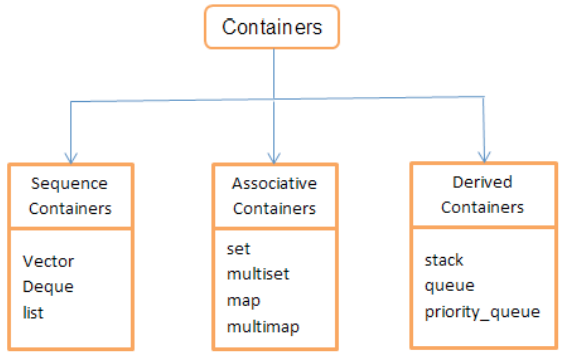
\includegraphics[width=300px]{images/6_STL/stl.png}
    \caption{STL containers hierarchy}
\end{figure}

\section{Iterators}
JCF (Java collection framework) and STL supports various kinds of collections/containers all of them uses iterators to provide uniform and linear access to elements of different collections.
In Java an iterator provides at least those two methods:
\begin{itemize}
    \item \verb|boolean hasNext()|;
    \item \verb|T next()|.
\end{itemize}

In general iterators are defined as nested classes (non-static private member classes) so each iterator instance is associated with an instance of the collection class.
Collection equipped with iterators have to implement the \verb|Iterable<T>| interface.

\subsection{Usage in Java}
Let's use an iterator of the example class \verb|BinTree|:
\begin{verbatim}
for(Iterator<Integer> it = myBinTree.iterator(); it.hasNext();){
    Integer i = it.next();
    // use i
}

for(Integer i : myBinTree){
    // use i
}
\end{verbatim}
java provides an enhanced for statement optimized for iterators, in particular that constructs accepts array of integers or something that implements \verb|Iterator<Integer>|.
Moreover the enhanced for on arrays is a bounded iteration.

\subsection{Usage in C++}
Conceptually they are the same but exploit different language features: in particular instead of methods they use the predefined C++ operators in order to be fully compatible with pointers:
\begin{verbatim}
for(vector<int>::iterator v = vec.begin(); v != vec.end(); v++){
    // use *v 
}
\end{verbatim}

\section{General structure}
STL relies on C++ namespaces in order to build it's structures, for example \\
\verb|std::vector<std::string>::iterator|.
Each class implicitly introduces a new namespace, so the iterator type assumes its meaning depending on the context.

Iterators are usually implemented as struct, which are classes with default public members, and implements a visit of the container keeping inside information about the state of the visit, which can be complex in the case of non linear structures such as trees or graphs.

\subsection{Complexity of operations on containers}
The library also specifies the guaranteed complexity for some operations:
\begin{figure}[H]
    \centering
    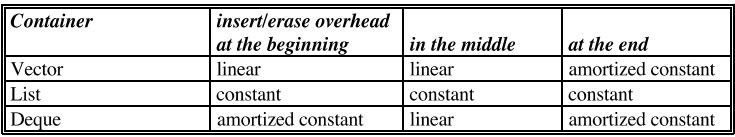
\includegraphics[width=300px]{images/6_STL/complexity.png}
\end{figure}
so let's consider the following code:
\begin{verbatim}
std::list<std::string> l;
...
quick_sort(l.begin(), l.end());
\end{verbatim}
since quick\_sort assumes random access we can't control the complexity of the algorithm.
In order to solve this problem the STL assumes that iterators implement all operations in constant time.

\subsection{Categories of iterators}
Containers may support different iterators depending on their structure:
\begin{itemize}
    \item Forward iterators: only dereferencing (\verb|operator*|) and pre/post-increment operators (\verb|operator++|);

    \item Input and Output iterators: like forwarding iterator but with possible issues in dereferencing the iterator (due to I/O operations);

    \item Bidirectional iterators: like forward iterators with pre/post-decrement (\verb|operator--|);

    \item Random access iterators: like bidirectional iterators but with integer sum and difference.
\end{itemize}
So we have 5 categories with decreasing requirements.
Each category has only those functions defined that are realizable in constant time, so not all iterators are defined for all categories: for example list can't have random access in constant time, so list won't implement random access iterators.

\subsubsection{Forward iterator}
Provides for one-directional traversal of a sequence, expressed with \verb|++|.
Moreover it has \verb|==|, \verb|!=|, \verb|*|, \verb|++|.

\subsubsection{Input and Output iterators}
Are like forward iterators but do not guarantee these properties of forward iterators:
\begin{itemize}
    \item iterators can be saved in order to keep going a second time;
    \item that it is possible to assign to the object obtained dereferencing an input iterator;
    \item that it is possible to read from the object obtained dereferencing an output iterator;
    \item that it is possible to test two output iterators for equality or inequality.
\end{itemize}

\subsubsection{Bidirectional iterators}
Provide methods for traversal in both directions using \verb|++| and \verb|--|.

\subsubsection{Random access iterators}
Provide methods for bidirectional traversal and for bidirectional long jumps using \verb|+=n| and \verb|-=n| and comparison through comparison operators.

\subsection{Iterator validity}
When a container is modified, iterators of it can become invalid and the result of operations on them could be not defined.
Relationship between operation and validity after it depends on the container type:
\begin{figure}[H]
    \centering
    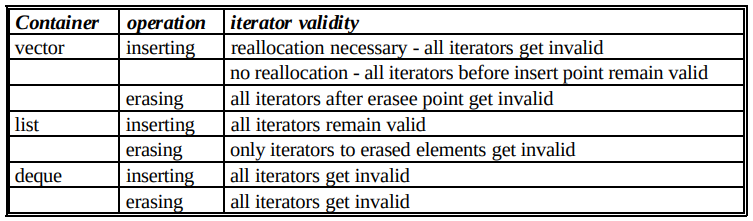
\includegraphics[width=300px]{images/6_STL/validity.png}
    \caption{Validity of iterators and operations}
\end{figure}

\subsection{Pros and cons}
Iterators provide a linear view of containers so we can't define algorithm which works on multiple dimensions, moreover if it is necessary to implement a custom visit of the container we can only re-define a new iterator with that custom algorithm.

Since there is no inheritance we have no relationship among iterators for different containers, this is a crucial point in order to exploit performance, both during run-time and during compilation because types are resolved at compile time so the compiler can produce better code using it's optimization.

In the end STL relies on coding conventions so when the programmer uses a wrong iterator the compiler will signal a bug inside the library, which is not the case, also those fails result in very lengthy error messages that most of the time are very tricky to understand and fix.

Moreover the generative approach taken by C++ compiler can bloat a lot the result and that bloat can be a problem if the working set of a process becomes too large!

\subsection{Inlining}
C++ standard has the notion of \emph{inlining functions} which is a form of semantic macros in which after a method invocation is type-checked then it is replaced by the method body.
Inline methods should be available in header files and can be labelled \verb|inline| or defined within class definition.

Inlining is not always used because the compiler tends to inline methods with small bodies and without iterations.

\subsection{Memory management}
STL abstracts from the specific memory model using \emph{allocators}.
All the information about the memory model is encapsulated in the \verb|Allocator| class and each container is parametrized by such allocator to let the implementation be unchanged when switching memory models (there is a default one used as default argument which implements STL's own memory management strategies). 
